\documentclass[12pt]{article}
\usepackage{url}
\usepackage[spanish, english]{babel}
\selectlanguage{spanish}
\usepackage[fixlanguage]{babelbib}
\selectbiblanguage{spanish}
\usepackage{url}
\usepackage[utf8]{inputenc}
\usepackage{float}
\usepackage{fullpage}
\usepackage{amsmath}
\usepackage{amssymb}
\usepackage{graphicx}
\usepackage{verbatim} 
\usepackage{caption, subcaption}
\usepackage{tikz}%Generar plots
\usepackage{pgfplots}%Generar plots
\pgfplotsset{compat=1.5}
\usepackage{pgfplotstable,filecontents}
\usepackage{booktabs}
\usepackage{lipsum}

\pgfkeys{/pgf/number format/.cd,fixed,precision=5}

\usepackage[titletoc, title]{appendix}
\addto{\captionsspanish}{\renewcommand*{\appendixname}{Anexo}}

\bibliographystyle{bababbrv}

\title{Segmentación de Piel}
\author{Jorge Bahamonde, Sebastián González\\
\small{\url{jbahamon@ug.uchile.cl}, \url{segonzal@dcc.uchile.cl}}}
\date{}

\begin{document}
\maketitle
\begin{comment}
\begin{abstract}
    El reconocimiento y clasificación de caracteres impresos es un método
    conocido para la digitalización de texto, de modo de poder realizar el
    almacenamiento, búsqueda y otros análisis de mejor forma.  El estudio y
    icomparación de diferentes descriptores es necesario en un área en que
    diversas variantes son propuestas en base a intuiciones. En particular, una
    clase importante de descriptores está compuesta por aquellos basados en
    nociones de concavidad. En este trabajo se estudiaron tres descriptores
    basados en concavidad para el caso de la clasificación de dígitos impresos.
    Se exploró (de forma limitada) el espacio de parámetros del clasificador
    utilizado (KNN). Posteriormente, se analizó la extensión de los resultados
    obtenidos en el caso de agregar mecanismos de división espacial en la
    obtención de los descriptores, buscando comparar el comportamiento de éstos.
\end{abstract}
\end{comment}
\section{Introducción}

%> grandes data sets (WWW) hacen posible soportar simples, eficientes algoritmos de aprendizaje.
%> dado una gran cantidad de datos, incluso simples reglas de aprendizaje arrojan buenos resultados
%> importante en el aprendizaje visual es la construccion de modelos de apariencia de la imagen desde datos de pixeles
% en paper "Statistical color models with application to skin detection" entrenaron un modelo de mix_of_gaussians con MUUUUUUCHOS dataz para clasificacion de piel
% analizamos la performance de MoG en el reconocimiento de piel en un set de 30 imagenes sacadas de la web

La masificación en el uso de la World Wide Web ha contribuido en la aparición de
grandes conjuntos de datos. La masividad de datos disponible soporta la
aparición de algoritmos simples y computacionalmente eficientes. Las grandes
colecciones de imágenes on-line permiten la construcción de modelos
estadísticos, caracterizando la apariencia de una imagen a través de la
información de sus pixeles.

La segmentación de piel es una aplicación útil del reconocimiento de patrones.
Es utilizada en el campo de la detección de personas y rostros, generalmente
para discriminar ambigüedades en la detección y reducir malas clasificaciones.
En el ámbito de la seguridad, ha sido usada en programas de control parental,
como herramienta de detección de contenido adulto en la web.

Estudiamos el segmentador de piel probabilístico propuesto por \emph{Jones y
Rehg} en \emph{Statistical color models with application to skin
detection}\cite{skin}. En particular analizamos el desempeño del método
\emph{Mixture of Gaussians}, al variar la razón de costo asociado a los falsos
positivos y falsos negativos ($\Theta$).

Utilizamos un set de datos de treinta imágenes, de las cuales la mitad fueron
encontradas en internet seleccionadas, considerando la tez de los sujetos. La
segunda mitad consiste en imágenes extraidas del dataset Pratheepan
\cite{dataset}.

\section{Descripción del Trabajo}

En este trabajo se realizó la evaluación de un algoritmo para el reconocimiento
de piel basado en modelos estadísticos de color. 

\subsection{Modelos de color}

Una forma de modelar una característica a detectar es mediante un modelo
estadístico sobre los colores de la imagen. Un pixel con cierto valor $rgb$ es
clasificado por uno de estos modelos como ser efectivamente piel si:

\begin{equation}
    \frac{ \mathbb{P} [ rgb|skin ] }{ \mathbb{P} [ rgb | \neg skin ] } \geq
    \Theta
\end{equation}

con $\Theta$ un umbral que puede ser descrito como función del costo de tener
falsos positivos y falsos negativos:

\begin{equation}
    \Theta = \frac{c_p \mathbb{P} [\neg skin]}{c_n \mathbb{P}[skin]}
\end{equation}

Ahora bien, las distribuciones $\mathbb{P} [ rgb|skin ]$ y $\mathbb{P} [ rgb | \neg
skin ]$ pueden ser determinadas de distintas formas. En el caso de este trabajo, se
utilizó un modelo que describe estas distribuciones como una combinación de
funciones gaussianas.

\subsection{Modelo basado en Mezcla de Gaussianas}

Una forma de modelar las distribuciones de probabilidad  $\mathbb{P} [ rgb|skin
]$ y $\mathbb{P} [ rgb | \neg skin ]$ es mediante una suma de funciones
gaussianas:

\begin{equation}
    \mathbb{P}[\mathbf{x}] = \sum\limits_{i=1}^N w_i
    \frac{1}{(2\pi)^{\frac{3}{2}} | \Sigma_i |^\frac{1}{2}} e^{-\frac{1}{2}
    (\mathbf{x} - \mathbf{\mu}_i)^{\text{T}} \Sigma_i ^{-1} (\mathbf{x} -
    \mathbf{\mu}_i)},
\end{equation} 

donde los valores $\mu_i$ y $\Sigma_i$ son las medias de cada gaussiana y las
correspondientes matrices (diagonales) de covarianza. Los valores $w_i$
determinan el peso que cada gaussiana ejerce en la mezcla. $N$ define la
complejidad del modelo, (ya que un mayor valor de $N$ resulta en más gaussianas
y por tanto un mayor número de grados de libertad) siendo un parámetro a
elección. 

Los autores de \cite{skin} entrenaron modelos para estimar ambas
distribuciones de probabilidad descritas, con lo que estos parámetros tienen
valores dados. Así, el trabajo se enfocó en variar el umbral de detección,
$\Theta$.

\subsection{Dataset utilizado}

Se construyó un pequeño \emph{dataset} compuesto por imágenes de dos tipos. Por
un lado, se recopilaron 14 imágenes buscando incorporar variaciones en
iluminación, tonos de piel y el nivel de detalle del fondo. Otras 16 imágenes
fueron tomadas del dataset utilizado en \cite{dataset} (junto con las
correspondientes \emph{ground truths}). Para cada imagen del
dataset generado, se obtuvo una imagen que identifica las zonas que son piel,
generándose así la \emph{ground truth} contra la que se comparó el rendimiento
del modelo estadístico. Cada imagen del dataset incluye al menos a una persona,
de modo que siempre se tiene piel por detectar.

\begin{comment}
\begin{figure}[H]
    \centering
    \subcaptionbox{Imagen del \emph{dataset}
    utilizado.}{\includegraphics[scale=0.9]{../images/nonbin/12.png}}
    \subcaptionbox{Perfil de piel utilizado como \emph{ground
    truth}}{\includegraphics[scale=0.9]{../images/bin/12.png}}
    \caption{Ejemplo del \emph{dataset} usado.}
\end{figure}
\end{comment}

\section{Resultados obtenidos}

Para evaluar el desempeño del modelo estudiado, se le utilizó para detectar piel
en las imágenes del dataset, contrastándolos con los perfiles de piel
etiquetados correctamente. 

Se definen, en este contexto: 

\begin{itemize}
    \item el \textbf{número de positivos ($P$)} como el número de pixeles en el dataset
        que corresponden a piel (según la \emph{ground truth});
    \item el \textbf{número de negativos ($N$)} como el número de pixeles en el dataset
        que no corresponden a piel;
    \item el \textbf{número de falsos positivos ($FP$)} como el número de
        pixeles en el dataset que el modelo identifica como piel, pero que no
        están etiquetados como tal en la \emph{ground truth};
    \item el \textbf{número de verdaderos positivos ($TP$)} como el número de
        pixeles en el dataset que el algoritmo identifica correctamente como
        piel;
    \item la \textbf{tasa de verdaderos positivos ($TPR$)} (también llamada
        probabilidad de detección correcta) como $\frac{TP}{P}$;
    \item la \textbf{tasa de falsos positivos ($FPR$)} (o probabilidad de
        detección incorrecta) como $\frac{FP}{N}$.
\end{itemize}

Así, el comportamiento de un modelo de detección como el estudiado puede ser
apreciado al comparar el comportamiento de la $FPR$ versus la $TPR$. La curva
definida por estas dos variables al modificar un tercer parámetro se denomina curva
ROC (del inglés \emph{receiver operating characteristic}). Esta curva muestra
cuán apropiado puede ser un modelo o algoritmo para ciertas aplicaciones, ya que
el costo de un falso positivo versus un verdadero positivo varía dependiendo del
contexto.

Se construyó una curva ROC a partir de los resultados obtenidos al utilizar el modelo de mezcla
de gaussianas en el dataset generado y la posterior comparación con la
\emph{ground truth}:


\begin{figure}[h]
    \centering
   % \includegraphics{digit}

\begin{tikzpicture}
\begin{axis}[
        title={Curva ROC},
	xlabel={False Positive Rate},
	ylabel={True Positive Rate},
	grid=major,
%	legend entries={$0.01$ , $0.1$,$0.5$},
%	legend style={at={(0,1)},anchor=north west},
]
\addplot table [scatter,x={FPR}, y={TPR}]{results100-ROC.csv};
\addplot table [scatter,x={FPR}, y={TPR}]{results500-ROC.csv};
\addplot table [scatter,x={FPR}, y={TPR}]{results1000-ROC.csv};
\addplot table [scatter,x={FPR}, y={TPR}]{results1500-ROC.csv};
\end{axis}
\end{tikzpicture}
    \caption{Curva ROC obtenida al variar el parámetro umbral $\Theta \in \{ 0.1,0.5,...,0.9,0.91,...0,99\}$.}
\end{figure}

Para ejemplificar de mejor forma el comportamiento del algoritmo, se presentan a
continuación algunos ejemplos en los que el modelo muestra diferentes grados de
efectividad.
\begin{comment}
\begin{figure}[H]
    \centering
   \hfill\subcaptionbox{Imagen original}{\includegraphics[scale=0.4]{../images/nonbin/05.png}}
   \hfill\subcaptionbox{\emph{GroundTruth}.}{\includegraphics[scale=0.4]{../images/bin/05.png}}
   \hfill\subcaptionbox{Output de \emph{Mixture of Gaussians} con $\Theta = 0.5$.}{\includegraphics[scale=0.4]{../done0.5/05.png}}
   \hfill\subcaptionbox{Output de \emph{MoG} con $\Theta = 0.9$.}{\includegraphics[scale=0.4]{../done0.9/05.png}}
   \caption{Imagen para la cual el modelo presenta un buen comportamiento}
\end{figure}

\begin{figure}[H]
    \centering
   \hfill\subcaptionbox{Imagen
   original}{\includegraphics[scale=0.3]{../images/nonbin/17.png}}
   \hfill\subcaptionbox{\emph{GroundTruth}.}{\includegraphics[scale=0.3]{../images/bin/17.png}}
   \hfill\subcaptionbox{Output de \emph{Mixture of Gaussians} con $\Theta =
   0.5$.}{\includegraphics[scale=0.3]{../done0.5/17.png}}
   \hfill\subcaptionbox{Output de \emph{MoG} con $\Theta =
   0.9$.}{\includegraphics[scale=0.3]{../done0.9/17.png}}
   \caption{Imagen para la cual el modelo presenta un comportamiento regular}
\end{figure}

\begin{figure}[H]
    \centering
   \hfill\subcaptionbox{Imagen
   original}{\includegraphics[scale=0.2]{../images/nonbin/09.png}}
   \hfill\subcaptionbox{\emph{GroundTruth}.}{\includegraphics[scale=0.2]{../images/bin/09.png}}
   \hfill\subcaptionbox{Output de \emph{Mixture of Gaussians} con $\Theta =
   0.5$.}{\includegraphics[scale=0.2]{../done0.5/09.png}}
   \hfill\subcaptionbox{Output de \emph{MoG} con $\Theta =
   0.9$.}{\includegraphics[scale=0.2]{../done0.9/09.png}}
   \caption{Imagen para la cual el modelo presenta un mal comportamiento}
\end{figure}
\end{comment}
\subsection{Discusión}

Se observa que, en general, el modelo alcanza resultados regulares. La curva ROC
obtenida muestra un desempeño ligeramente menor que el alcanzado por los autores
de \cite{skin}. En particular, el modelo parece presentar un menor rendimiento
cuando el fondo es más bien simple, logrando, por el contrario, un mejor
comportamiento en casos en los que el fondo posee elementos rojizos (como
madera, por ejemplo). 

Bajo condiciones de iluminación normales, el modelo parece presentar una alta
sensibilidad, si bien no una alta especificidad (lo que se observa rambién en la
curva ROC obtenida). Se aprecia, además, que se aquellas imágenes en las que el
fondo presenta colores similares a la piel, como es esperable. En el otro
extremo, imágenes con iluminación coloreada fallan considerablemente,
presentando una bajísima cantidad de verdaderos positivos.

\section{Conclusiones}

%Observamos que nuestros resultados son peores que los de "la gente del papaer"

%creemos que los resultados mejorarian de agregar imagenes sin piel que detectar

%las imagenes que elegimos estan sucias: colores de fondo. -> fallan tanto

El trabajo realizado permitió observar un peor desempeño de
\emph{Mixture of Gaussians} sobre el conjunto de datos construido que el
obtenido por \emph{Jones y Rehg}. Esto puede ser atribuido a la selección de
imágenes que constituyen el dataset utilizado. A diferencia de Jones y Rehg, las
imágenes utilizadas siempre tienen una persona en ellas, lo que induce una menor
relación de negativos. Esto, a su vez, hace que los falsos negativos se vean más
representados. Es posible que agregar imágenes iluminadas, de buena calidad e
incluso imágenes en las que no hay presencia de piel, contribuirían a mejorar el
desempeño de \emph{MoG} en un dataset de este tamaño.

Por otro lado, se aprecia que existen diferentes tipos de error. En ciertos
casos, existen muchos pixeles dispersos detectados como piel esparcidos por la
imagen. En este caso, podría ser interesante aplicar algún mecanismo de
detección de \emph{blobs} de modo de descartar este tipo de errores. Otros casos
corresponden a la identificación de ciertas telas y texturas como piel, en los
que combinar con técnicas como \emph{local binary patterns} podrían resultar en
un mejor desempeño. De todos modos, la conveniencia de complementar el modelo
con estas herramientas depende del contexto de uso.

A pesar de sus limitaciones, \emph{MoG} resulta útil como herramienta para la
depuración de ambigüedades en métodos más complejos de detección de rostros y de
personas. Esto ya que, una vez detectada una ambigüedad, es posible realizar
\emph{MoG} sobre la zona en cuestión y discriminar a partir de la presencia de
piel.

\selectlanguage{spanish}
\selectbiblanguage{spanish}

\bibliography{./informe}

\begin{appendices}

\section{Tasas de falsos positivos y verdaderos positivos obtenidas}

\begingroup
\centering
\pgfplotstabletypeset[col sep=tab,
%     columns={theta,FPR,TPR},
     display columns/0/.style={column name=$\Theta$},
     display columns/1/.style={column name=\emph{FalsePositiveRate}},
     display columns/2/.style={column name=\emph{TruePositiveRate}},
     every head row/.style={before row=\toprule,after row=\midrule},
     every last row/.style={after row=\bottomrule},
    ]{results100-ROC.csv}
\captionof{figure}{Tasas de falsos positivos y verdaderos positivos obtenidas.}\label{fig:f}
\endgroup


\end{appendices}


\end{document} 
